%%% initial
\documentclass[ukrainian,14pt,utf8,
%pointsection, % це хз для чого
nocolumnsxix,
nocolumnxxxi,
nocolumnxxxii,
floatsection, %підпис плаваючих об'єктів згдіно номера розліду (таблиці, рисунки)
hpadding=5mm, %відстань до рамки зліва, справа
vpadding=5mm %відстань до рамки зліва, справа
]{eskdtext}

%%% for working with math
%\usepackage{amsmath}
%\usepackage{amssymb}

%%% for working some LaTeX packages
\usepackage{xecyr}

%%% for fonts
\usepackage{xltxtra}
%%% Times New Roman - main font
\setmainfont[Mapping=tex-text]{Times New Roman}
%%% Courier New - fot math
\setmonofont[Scale=MatchLowercase]{Courier New}

%%% for ---, --, << >> и т.п.
\defaultfontfeatures{Mapping=tex-text}

%%% ukrainian text
\usepackage{polyglossia}
\setdefaultlanguage{ukrainian}
\newfontfamily\ukrainianfont{Times New Roman}

%%% for words wrapping
%\XeTeXinterchartokenstate=1
%\XeTeXcharclass `\- 24
%\XeTeXinterchartoks 24 0 ={\hskip\z@skip}
%\XeTeXinterchartoks 0 24 ={\nobreak}

% для абзацу %
\usepackage{indentfirst}

% code highlighting %
\usepackage{listings}
\lstset{
language=Java,
basicstyle=\footnotesize\sffamily,
numbers=left,
numberstyle=\tiny,
frame=tb,
columns=fullflexible,
showstringspaces=false,
breaklines=true 
}

% automaticaly wrap to other line
\sloppy
%\usepackage{setspace}
%\onehalfspacing
\linespread{1.5}

%%% for graphix
\usepackage{graphicx}
\graphicspath{{images/}} %path to images
%%% titile for pictures
\addto{\captionsukrainian}{\renewcommand{\figurename}{Рисунок}}


%%% for internet ulrs
\usepackage{url}

%%% subtitiles(\subsubsection) don't show in article
%\setcounter{tocdepth}{2}

%%% new section from new page
\let\stdsection\section
\renewcommand\section{\newpage\stdsection}

%%% плаваючі обєкти підпис
%\renewcommand\section{\newpage\stdsection}

%%% Numering subtopics begin with B (B.1)
%\makeatletter
%\renewcommand\thesubsection{\ifnum\c@section=0{В.\arabic{subsection}}\else{\arabic{section}.\arabic{subsection}}\fi}
%\makeatother

%%% for coloring rows
\usepackage[table]{xcolor}

%%% для розриву таблиць 
\usepackage{longtable}
%\usepackage{eskdgraph}






\ESKDtitle{ Аналіз розробки програмного алгоритмічного забезпечення багатофункціональної корпоративної системи для сумісної роботи, управління документами і проектами }
\ESKDdocName{\uppercase{Звіт з переддипломної практики}}
\ESKDgroup{ІНФТУНГ ПЗ-07-1}

\ESKDauthor{ Бойчук Я.В. }
\ESKDchecker{ Бандура В.В. }
\ESKDsignature{ ПП.ПЗ 03.00.00.000 ПЗ }

%%finixg ukrainian languale%%
\renewcommand{\ESKDcolumnXfIname}{Розробив}
\renewcommand{\ESKDcolumnXfIIname}{Перевірив}
\renewcommand{\ESKDcolumnXfIVname}{Т.контр}
\renewcommand{\ESKDcolumnXfVname}{Н.контр}
\renewcommand{\ESKDcolumnXfVIname}{Затв.}

\renewcommand{\ESKDcolumnIVname}{Літ.}
\renewcommand{\ESKDcolumnVIIIname}{Аркушів}
\renewcommand{\ESKDcolumnXVIIname}{Підпис}
\renewcommand{\ESKDcolumnXVname}{Арк.}

%%fix ESKDTitle font
%%FIXME change for row, now for font
\renewcommand{\ESKDfontVsize}{%
\ESKDfontSetBaseLineStretch
\fontsize{10pt}{8pt}\selectfont\ESKDfontShape}

%%space after text
\setlength{\ESKDsectionSkipBefore}{-7mm \@plus -3mm \@minus -2mm}
\setlength{\ESKDsectionSkipAfter}{7mm \@plus 1mm \@minus 2mm}
\setlength{\ESKDsubsectionSkipBefore}{-7mm \@plus -3mm \@minus -2mm}
\setlength{\ESKDsubsectionSkipAfter}{7mm \@plus 1mm \@minus 2mm}
\setlength{\ESKDsubsubsectionSkipBefore}{-7mm \@plus -3mm \@minus -2mm}
\setlength{\ESKDsubsubsectionSkipAfter}{7mm \@plus 1mm \@minus 2mm}

%%font size for section (&&sub)
\renewcommand{\ESKDsectionStyle}{\centering\normalfont\bfseries\MakeUppercase}
\renewcommand{\ESKDsubsectionStyle}{\centering\normalfont\bfseries}
\renewcommand{\ESKDsubsubsectionStyle}{\centering\normalfont\bfseries}




        



\begin{document}
\fontsize{14}{14pt}\selectfont

\maketitle


\tableofcontents


%\section*{Вступ}
%\addcontentsline{toc}{section}{Вступ}
%Текст вступу
%

\section{Вступ}
В нас час важливою економічною точкою опори для будь-якої комерційної організації є наявність певних факторів, які визнають чітку позицію компанії на ринку. До всіх цих чинників можна віднести багато варіантів, зокрема:
\begin{enumerate}
\item капітал підприємства;
\item матеріальна база;
\item технічна база;
\item кваліфікований персонал;
\item місце підприємства на внутрішньому і зовнішньому ринку;
\item наявність сучасних засобів виробництва та ведення бізнесу;
\item та інші.
\end{enumerate}

Тому кожний розділ ведення бізнесу повинний бути детально розглянутий та впроваджений у життя. 
Але якщо подивитися із точки зору програмного забезпечення, то на даному етапі розвитку цивілізації, якісне ПЗ відіграє напевно найбільш важливу роль. 
Адже не можливо зараз утримувати всі дані в паперовому вигляді, не можливо відсилати друковані листи, чи спілкуватися тільки по телефоні і взнавати новини компанії тільки при зустрічі. 
У наш стрімкий час розвитку, новини міняються із колосальною швидкістю, тому встигнути за всім просто не можливо без певного програмного продукту. 
Уявіть собі інформатор, який сповіщає будь-які для Вас новини чи корисну інформацію в зручний для Вас час, при цьому вміє фільтрувати і аналізувати дані із попередніх запитів. 
Також на даний момент важко уявити не можливість спільної роботи над документами, над електронними таблицями. 
Дані технології вже давно використовуються людьми і підприємствами, починаючи від найменших де працює двоє людей, до величезних із кількістю працівників більше ста тисяч. 
Але для цього всього використовуються дуже багато технологій, які важко налаштувати і потребують великих витрат на підтримку.
Тому було розроблено багато сервісів і додатків, які полегшують роботу в мережі для підприємств.
\par Дане ПЗ використовується у всіх нішах нашого життя, починаючи від шкіл і лікарень, закінчуючи величезними корпораціями з будівництва космічних кораблів. 
Тому розробити універсальний продукт, який забезпечить всі вимоги, просто не можливо. 
Для кожної сфери існують свої нюанси.
\par Цікавою нішею для дослідження стало корпоративне програмне забезпечення для малого і середнього бізнесу.
 На даний момент існує багато програмних продуктів для комерційних цілей, проте вони здебільшого розраховані на великі корпорації і підприємства.
Тому використання їх для менших фірм просто не доцільно, або дуже складно із фінансової сторони (витрати на підтримку передують вигоді).
Як відомо, на ринку до цих пір зберігається тенденція на попит на корпоративне програмне забезпечення, яке б відповідало вимогам малого і середнього бізнесу, і в той же час було практично придатним для використання у великих корпоративних цілях

%TODO придумати назву заголовку. Може включити у підрозділ вступ
\section{Огляд програмного продукту}
Розглянемо більш детально пункт про наявність сучасних засобів ведення бізнесу. 
Кожна компанія, завжди стикається із проблемою ведення обліку працівників, ведення обліку фінансів, спільної роботи над документами та іншим.
Також є величезна і невід'ємна потреба у спільному доступі до документів, до корпоративного календаря, до блогу користувачів, до електронних таблиць та інформаційної дошки.
\par Портал підприємства (також відомий як enterprise information portal (EIP) або корпоративний портал) є основою для інтеграції інформації, людей і процесів в рамках організації. 
Це дає змогу забезпечити єдину точку доступу, часто у вигляді веб-інтерфейсу і призначеної для агрегування та персоналізації інформації за допомогою конкретних програмних додатків. Однією відмінною рисою корпоративних порталів є децентралізоване внесення контенту та управління, яка зберігається на віддаленому сервері та постійно оновлюється.
%TODO змінити якось =)
\subsection{Історичний огляд коропоративної сфери}
В середині 1990-х років появилися громадські такі веб-портали як AltaVista, AOL, Excite і Yahoo!. 
Вони забезпечували користувачів певним набором функцій (наприклад новини, електронна пошта, погода, котирування акцій і пошук), які часто були представлені у вигляді автономного порталу.
Незабаром підприємства усіх типів і форм почали бачити необхідність аналогічного функціоналу для їх різноманітних потреб, проте із єдиною точкою доступу.
До кінця 1990-х років, виробники програмного забезпечення почали розробляти веб-портали для різних підприємств. 
Ці програмні пакети були розроблені таким чином, щоб підприємства могли легко розгортати свої власні налаштування корпоративного порталу та доповнювати його своїми додатками.
Перші постачальники комерційних веб порталів з'явилися в 1998 році, це були такі фірми як: Epicentric, Plumtree  та Viador. 
Ці фірми були основними гравцями на ринку, проте ситуація змінилася в 2002 року, коли на ринок почали виходити постачальникики серверних аплікацій, такі як BEA, IBM, Passageways, Oracle Corporation and Sun Microsystems.
Підприємства можуть вибрати для своїх цілей декілька порталів, що базується на основі їх бізнес-структури та стратегічної спрямованості.
У 2003 році розробники Java-порталів випустили стантарт, відомий як JSR-168. 
Він повинен був визначити API для взаємодії між корпоративних порталів та портлетів.
Постачальники програмного забезпечення почали розробляти JSR-168 сумісні портлети, які можуть бути розгорнуті на будь-якому JSR-168 сумісному корпоративному порталі. 
Другий ітераційний стандарт JSR-286 є остаточним на даний момент і випущений 12 червня 2008 року.

\subsection{Портлети}
Портлет - це змінний компонент інтерфейсу веб-порталу (елемент веб-сторінки), який можливо певним чином підключити до порталу.
Портлет містить в собі фрагменти розмітки, які вбудовуються в сторінку порталу. 
Найчастіше сторінка порталу представляється у вигляді набору портлетів, які взаємодіють між собою. 
Таким чином, портлет (або сукупність портлетів) представляється у вигляді єдиного веб-додатку, розміщеного на порталі. 
Приклади портлетів можуть бути наступними: електронна пошта, повідомлення про погоду, фінансовий стан, останні новини і тому подібне.
Завдяки існуючим стандартам розробники можуть створювати портлети, що легко вбудовуються в будь-який портал, який слідує стандартам і правилам.
\par Існує протокол WSRPasdasdasd a , що забезпечує стандарт веб-сервісів, що дозволяє автоматично вбудовувати віддалено запущені портлети з різних джерел.
Специфікація Java-портлетів JSR168 дає можливість взаємодіяти між собою портлети з різних веб-порталів. 
Ця специфікація визначає безліч API для взаємодії контейнерів портлетів і дає різні адреси областей персоналізації, подання та безпеки.
Існує безліч постачальників комерційних контейнерів портлетів. 
Як відомо лідирують у цій галузі IBM, Oracle, Vignette. 
Реалізації від цих постачальників мають додаткові розширення і налаштування, проте деякі із ним можуть бути не затверджені стандартами. 
Крім того, є портали з відкритим вихідним кодом, що підтримують JSR168, такі як корпоративний портал Apache Jetspeed-2 або eXo Portal.
\subsubsection{Apache Pluto}
Розглянемо на прикладі один з найбільш вдалої реалізації стандартку портлетів JSR168 - це Apache Pluto.
Портлет працює всередині контейнера портлетів (Pluto).
Цей контейнер містить портлет з необхідним середовищем для подальшого виконання.
Контейнер портлетів керує життєвим циклом всіх вікон порталу та надає інтерфейси для портлетів, котрі викликаються всередині нього.
Контейнер також запускає методи на виконання із доступних цільових користувацьких сторінок, і взаємодіє із сторінками порталу.

        \begin{center}
		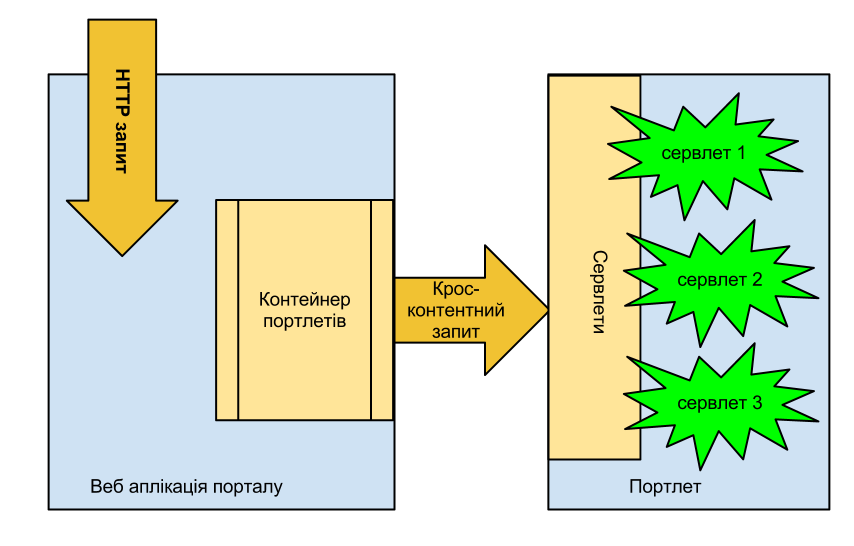
\includegraphics[width=1.00\textwidth]{pluto.png}
		\captionof{figure}{Принцип роботи <<Pluto>>}
	\end{center}

На наступному малюнку зображено архітектурні компоненти аплікації Pluton 2.0. 
\par В даному випадку, Pluton вбудований безпосередньо в корпоративний портал. 
Потім через перехресний запит (через веб-додатки) відбувається відправлення запиту для відображення вмісту портлету, який як правило знаходяться в різних додатках на порталі і в контейнерах. 

\section{Основні компоненти аплікації}
%TODO список для більшості сторінок =)



\subsection{Система керування вміcтом}
Система управління контентом (content management system - CMS) дозволяє публікувати, редагувати і змінювати вміст веб-сторінок, а також обслуговувати портал з центральної сторінки. 
При цьому надається набір процедур, що використовуються для управління робочим процесом у середовищі для спільної роботи.
Вони можуть бути ручні або комп'ютеризовані (в автоматичному режимі).
\subsubsection{Головні функції CMS}
До основних функцій можна віднести наступні пункти:
\begin{enumerate}
\item можливість великій кількості людей ділитися інформацією і робити свій вклад в розвиток порталу;
\item контроль доступу до даних на основі ролей користувачів (наприклад визначити роль, яка має тільки права на перегляд інформації, або ж редагування, публікацію тощо);
\item пошук і поширення інформації між користувачами;
\item змешення дублікацій на вході;
\item спрощене керування корпоративними додатками;
\item відносно легка комунікація між користувачами.
\end{enumerate}

\subsubsection{Типи даних та їх використанням}
У CMS дані можуть бути представлені як правило у будь-якій формі: документи, відео, тексти, фотографії, номери телефонів, наукові дані і тому подібне. 
CMS часто використовуються для зберігання, управління, перегляду і публікації документів. 
Також досить поширине використання в якості центрального сховища у зв'язці із централізованою системою контролю версій, що є однією із переваг CMS.
\subsubsection{Управління корпоративною інформацією}
Enterprise Content Management (ECM) - управління інформаційними ресурсами підприємства або управління корпоративною інформацією.
В даному контексті інформація (контент) передбачається як слабо структурована одиниця - це можуть бути файли різних форматів, електронні документи з різними наборами полів і т. п.
За визначенням ECM - це стратегічна інфраструктура і технічна архітектура для підтримки єдиного життєвого циклу неструктурованої інформації різних типів і форматів. 
ECM-системи складаються з додатків, які можуть взаємодіяти між собою, а також використовуватися і продаватися самостійно. 
\par Всі сучасні ECM-системи визначають такі ключові компоненти:
\begin{enumerate}
\item управління документами --- довгострокове архівування, автоматизація політик зберігання та відповідності нормам регулюючих органів, забезпечення відповідності законодавчим та галузевим нормам;
\item управління веб-контентом (WCM) --- автоматизація ролі веб-майстра, управління динамічним контентом і взаємодією між користувачами;
\item  управління мультімедіаконтентом (DAM) --- управління графічними, відео та аудіофайлами, різними маркетинговими матеріалами, наприклад, флеш-банерами, рекламними роликами;
\item управління знаннями (Knowledge Management) --- підтримка систем для накопичення та доставки релевантної для бізнесу інформації;
\item документо-орієнтоване взаємодія (співробітництво) --- спільне використання документів користувачами та підтримка проектних команд.
\end{enumerate}

%TODO якщо буде мало тексту, вставити http://en.wikipedia.org/wiki/Enterprise_content_management
%\subsubsection{Компоненти ECM} 

\subsection{Система управління документами}
Система управління документами  (англ. DMS - Document management system) - комп'ютерна система (або набір комп'ютерних програм), що використовується для відстеження та зберігання електронних документів і / або образів (зображень та інших артефактів) паперових документів.
Дане поняття тісно пов'язане з концепцією Content Management System (система керування вмістом) і зазвичай розглядається як компонент Enterprise Content Management System (CMS рівня підприємства).
У загальному випадку системи управління документами (DMS) надають можливість зберігання, ведення контролю версій, позначення метаданими і безпеку по відношенню до документів, а також індексування і розвинені можливості пошуку документів.
\subsubsection{Метадані}
Метадані зазвичай зберігаються для кожного документа. 
Метадані, наприклад, можуть включати дату занесення документа в сховище і код користувача, котрий виконав зміни до файлу. 
Система управління документами також може витягувати метадані з документа автоматично або запитувати їх у користувача. 
Деякі системи надають сервіс оптичного розпізнавання тексту відсканованих документів, або можливість витягувати текст з електронних документів. 
Використовуючи опрацьований текст система дозволяє здійснювати пошук документа за ключовими словами всередині самого документа.

\subsubsection{Інтеграція }
Багато систем управління документами намагаються інтегрувати функцію управління документами безпосередньо в різні додатки, дозволяючи користувачеві отримувати документ відразу зі сховища системи управління документами, робити які-небудь модифікації, і зберігати його назад в сховище в якості нової версії, і все це проробляти в одному додатку, не виходячи з нього. 
Дана інтеграція в основному доступна для офісних пакетів і поштових клієнтів або для програмного забезпечення, призначеного для групової або колективної роботи. 
Інтеграція зазвичай має на увазі використання таких відкритих стандартів як: ODMA, LDAP, WebDAV і SOAP.

\subsubsection{Захоплення тексту}
Під захопленням тексту мається на уазі переведення паперових документів в цифровий варіант за сканерів та МФУ.
Також часто використовується програмне забезпечення для оптичного розпізнавання тексту, щоб конвертувати цифрові зображення в текст.

\subsubsection{Індексування}
Індексування надає можливість класифікувати документи за допомогою метаданих і індексування словникового тексту, який було витягнутого з документа.
Індексація існує для підтримки розвинених можливостей пошуку документів. 
Одна з головних умов швидкого та якісного пошуку - це створення індексу документа.

\subsubsection{Сховище}
Основне призначення це для зберігання електронних версіх документів. 
Сховище документів також включає в себе і керування тими ж документами, котрі воно зберігає.
Також сховище забезпечує міграцію з одного носія на інший і забезпечує цілісність даних.
Сховище документів може бути як файлове, так і сховище у вигляді СУБД (бази даних). 
У свою чергу, сховище документів в СУБД може бути як в одній базі даних, так і в окремо розподілених базах даних.
        

\section{Програмне забезпечення спільної роботи}
Програмне забезпечення спільної роботи (англ. collaborative software, groupware, workgroup support systems, group support systems) - програмне забезпечення створене з метою підтримки взаємодії між людьми, котрі спільно працюють над вирішенням деяких спільних завдань. 

\subsubsection{Огляд}
Програмне забезпечення для спільної роботи --- це область, яка в значній мірі перекривається з областю CSCW (англ. computer-supported cooperative work (CSCW)).
Часто вважається що ці області еквівалентні, хотя з іншого боку програмне забезпечення для спільної роботи є підчастиною CSCW.
Сюди відносяться такі системи як: електронна пошта, календарі, текстовий чат, вікі сторінки, корпоративні закладки, блог.
Оскільки ПО спільної роботи відноситься до технологічних елементів CSCW, системи спільної роботи стають корисним аналітичним інструментом у вивченні поведінкових і організаційних параметрів, пов'язаних з більш широкою сферою CSCW.

%FIXME забрати перекладений текст, хтось колись в неті перекладав
\subsubsection{Види взаємодії}
Можна зустріти кілька різних визначень спільної роботи (англ. - collaboration) в застосуванні до інформаційних технологій. Деякі з них виправдані, інші ж настільки великі, що починають втрачати будь-який сенс.
Для того щоб бути впевненим що обрані технології підходять для конкретних потреб, необхідно розуміти відмінності в способах взаємодії людей один з одним.
Є три основні шляхи, по яких здійснюється взаємодія між людьми: 
\begin{enumerate}
\item діалог;
\item здійснення угоди;
\item співробітництво.
\end{enumerate}

\par Діалог - це обмін інформацією між одним або кількома учасниками, основна мета якого полягає у з'ясуванні їх позицій і встановлення взаємин. 
Відбувається вільний обмін інформацією без будь-яких обмежень. 
Для підтримання діалогу цілком підходять звичайні комунікаційні технології, такі як телефон, миттєві повідомлення та електронна пошта.
\par Укладення угоди передбачає обмін якимись сутностями, і ця процедура зазвичай проводиться за добре певними правилами і передбачає зміну відносин між учасниками. Наприклад, один з учасників угоди обмінює гроші на товари і стає покупцем. Новий статус учасників операції та обмінюваних сутностей потрібно зберегти в будь-якому надійному сховищі. Такі операції добре обслуговуються системами управління транзакціями. 
\par Співпраця полягає в тому, що його учасники обмінюються якимись загальними сутностями (на противагу угоді, коли предмет обміну належить лише одному учаснику). 
Як приклад можна привести просування нової ідеї, створення нової конструкції, досягнення спільних цілей. 
При цьому самі сутності досить розпливчасті і невизначені. 
Таким чином, технології для забезпечення спільної роботи теж повинні бути достатньо гнучкими. 
Вони повинні включати в себе управління документами, кошти для ведення обговорень з можливістю сортування за темами, можливість відновити історію внесених змін та багато іншого.
 

\subsection{Корпоративна пошта}

\subsection{Онайл офіс}
\subsection{Корпоратиний блог}
\subsection{Розподілене управління контентом}

\section*{Висновок}
\addcontentsline{toc}{section}{Висновок}
Текст висновку

%%% Bibliography
\catcode`"\active\def"{\relax}
\bibliographystyle{gost780s}
\bibliography{bibliography}{}
\end{document}

